\documentclass{article}
\usepackage{graphicx} % Required for inserting images
\usepackage[
backend=biber,
style=numeric,
sorting=ynt
]{biblatex}
\usepackage{todonotes}
\usepackage{caption}
% \usepackage{fontspec}

% \setmainfont{Times New Roman}
% \setlength{\parskip}{1em}

\addbibresource{bibliography.bib}

\begin{document}

\title{Making A Roguelike Engine with SvelteKit}
\author{Kutay Güler}
\date{December 2023}

\todo{school info}

\maketitle
\tableofcontents

\section{Introduction}
In every software project, whether it is a game, a game engine or a simple web application, there is a property which can cause a project to get derailed or follow a steady pace to its ultimate destination, and that property is called “scale.”\\ 

Although getting derailed is a negative phrase, in the context of software engineering it could be a necessity, especially for game engines. Most popular game engines today have massive codebases with many people working on them, because their promise is the ability to create any type of game at any scale with only one tool. This is like inventing a train that can fly, travel underwater, go to the moon and of course, slide on iron rails. By its nature, it should derail from time to time.\\

It sounds like there are only upsides to this invention since it can go anywhere but upon closer inspection, we can conclude that it is incorrect. The different environments this train will travel through will require many edge cases which will increase the literal size of the train and its maintenance cost. As for passengers, the experience will require some time to get used to and first timers will be definitely intimidated.\\ 

This project’s aim is to create a straightforward train with its blueprints open to the public, that is, an open-source game engine specifically designed for roguelikes. The target audience is people who want to make roguelike games without having to learn coding but there will be grounds for programmers too.\\ 

\subsection{Design Philosophy}
Roguelighter aims to make the engine as simple as possible and reducing the user input to minimum, while keeping the engine flexible. If there was a trade-off to be made between simplicity and flexibility, then simplicity would drive the development. 

Speaking of making things simpler, one could think that a game engine that promises simplicity should have a visual programming language rather than a textual one. We think the opposite is true.

\subsubsection{Why visual programming is bad}
A visual programming language or block coding is a programming language that lets users create programs by manipulating program elements graphically rather than by specifying them textually.\\

The problem with this approach is that you have created one more layer of abstraction both for the consumer and the maintainer of the language. Consumer now has to learn the specific nodes rather than learning the language itself and organize the nodes in a 2D space to his/her liking (The textual equivalent of organizing nodes would be not using a code formatter to format your code, which is an obvious waste of time). Maintainer should create readable and accessible nodes for every language feature which doubles his work to produce anything. The brevity of text is traded for the superficial ease of conveying information via verbose graphical elements. \todo{citation needed}.

\subsubsection{Godot Engine and VisualScript}
Godot Engine, a free, open-source general purpose game engine has discontinued its visual scripting system in its latest stable version. There are multiple reasons why they discontinued it but the crucial answer for Roguelighter's development philosophy was this:\\

"For a lot of potential users that wanted this feature, they found out GDScript was a great fit and they pretty much ended up preferring it over VisualScript. They did not expect to find GDScript to be so easy to learn and use (even if they did not have prior programming knowledge), given none of the popular engines of the time offered this type of high level scripting. For many of these users, Godot ended up being a tool to learn programming instead."

\begin{minipage}{\linewidth}
    \centering
    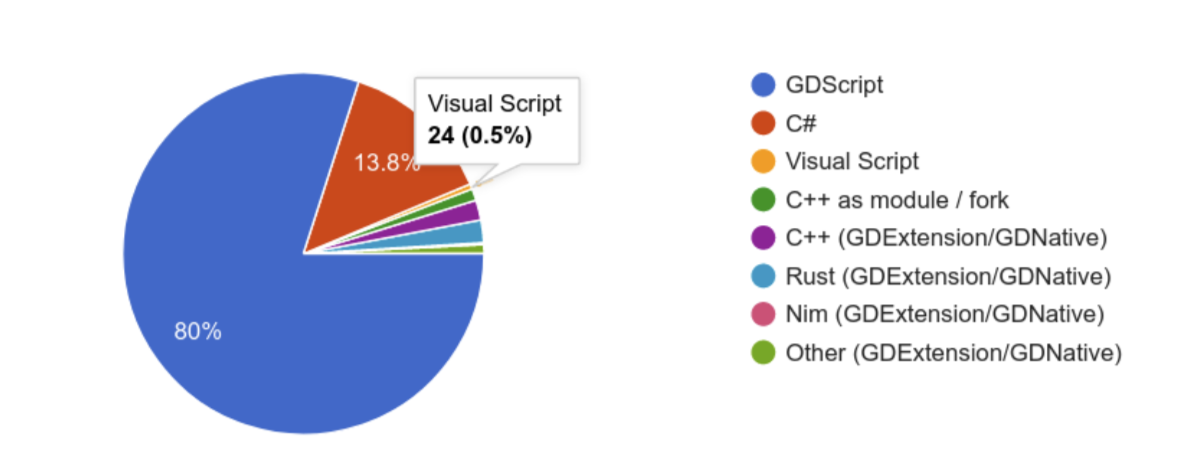
\includegraphics[width=1\textwidth]{godot-statistics.png}
    \captionof{figure}{Godot programming language statistics}
\end{minipage}\\\\

Once a programming language is easy to use, there is very little reason to make it visual.

\subsubsection{CDD (Configuration Driven Development)}
Roguelighter does not intend to invent a language because it does not have to. CDD is a way of using modularity to build a loosely coupled set of components that are then composed together using a common interface. This way, making a Roguelighter game will be like filling in the blanks of a document, speaking a natural language.

\subsection{Roguelike}
The term roguelike originated in a forum discussion to find an umbrella term for games that were similar to each other at the time. After three weeks of discussion, the “granddaddy of these games” Rogue, was appended with “-like” suffix to turn it into a game genre that we still use today \cite{roguelike-term}.\\ 

\begin{minipage}{\linewidth}
    \centering
    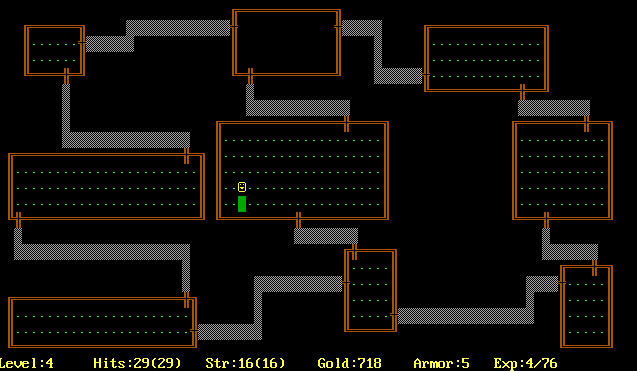
\includegraphics[width=1\textwidth]{rogue.png}
    \captionof{figure}{A screenshot from the Rogue (1980) game}
\end{minipage}\\\\

Many roguelike games were released in the upcoming years, so it was time to define what a roguelike game is more concretely. In 2008, the International Roguelike Development Conference was held in Berlin, and gave birth to the Berlin Interpretation \cite{berlin}.\\

\subsection{Berlin Interpretation}

Text below is the formatted version of the original Berlin Interpretation text. All the content has been kept exactly the same.

\subsection*{Preamble}

This definition of "Roguelike" was created at the International 
Roguelike Development Conference 2008 and is the product of a 
discussion between all who attended. The definition at 
http://www.roguetemple.com/roguelike-definition/ was used as the 
starting point for the discussions. Most factors are newly phrased, 
new factors have been added, some factors have been removed.

\subsection*{General Principles}
 
"Roguelike" refers to a genre, not merely "like-Rogue". The genre is 
represented by its canon. The canon for Roguelikes is ADOM, Angband, 
Crawl, Nethack, and Rogue.\\
 
This list can be used to determine how roguelike a game is. Missing 
some points does not mean the game is not a roguelike. Likewise, 
possessing some points does not mean the game is a roguelike.\\  
 
The purpose of the definition is for the roguelike community to better 
understand what the community is studying. It is not to place 
constraints on developers or games.\\

\subsection*{High value factors}
\begin{itemize}

\item\textbf{Random environment generation:}
The game world is randomly generated in a way that increases 
replayability. Appearance and placement of items is random. 
Appearance of monsters is fixed, their placement is random. 
Fixed content (plots or puzzles or vaults) removes randomness. 

\item\textbf{Permadeath:} 
 You are not expected to win the game with your first character. You 
start over from the first level when you die. (It is possible to save 
games but the savefile is deleted upon loading.) The random 
environment makes this enjoyable rather than punishing. 

\item\textbf{Turn-based:}
Each command corresponds to a single action/movement. The game is not 
sensitive to time, you can take your time to choose your action.   

\item\textbf{Grid-based:} 
The world is represented by a uniform grid of tiles. Monsters (and 
the player) take up one tile, regardless of size. 

\item\textbf{Non-modal:} 
Movement, battle and other actions take place in the same mode. Every 
action should be available at any point of the game. Violations to 
this are ADOM's overworld or Angband's and Crawl's shops. 

\item\textbf{Complexity:} 
The game has enough complexity to allow several solutions to common 
goals. This is obtained by providing enough item/monster and item/item 
interactions and is strongly connected to having just one mode. 

\item\textbf{Resource management:} 
You have to manage your limited resources (e.g. food, healing potions) 
and find uses for the resources you receive. 

\item\textbf{Hack'n'slash:}
Even though there can be much more to the game, killing lots of 
monsters is a very important part of a roguelike. The game is player- 
vs-world: there are no monster/monster relations (like enmities, or 
diplomacy).  

\item\textbf{Exploration and discovery:} 
The game requires careful exploration of the dungeon levels and 
discovery of the usage of unidentified items. This has to be done anew 
every time the player starts a new game.

\end{itemize}

\subsection*{Low value factors} 
\begin{itemize}
    \item \textbf{Single player character:}
    The player controls a single character. The game is player-centric, 
    the world is viewed through that one character and that character's 
    death is the end of the game. 
    
    \item \textbf{Monsters are similar to players:}
    Rules that apply to the player apply to monsters as well. They have 
    inventories, equipment, use items, cast spells etc. 
    
    \item \textbf{Tactical challenge:}
    You have to learn about the tactics before you can make any 
    significant progress. This process repeats itself, i.e. early game 
    knowledge is not enough to beat the late game. (Due to random 
    environments and permanent death, roguelikes are challenging to new 
    players.) 
    
    The game's focus is on providing tactical challenges (as opposed to 
    strategically working on the big picture, or solving puzzles). 
    
    \item \textbf{ASCII display:}
    The traditional display for roguelikes is to represent the tiled world 
    by ASCII characters. 
    
    \item \textbf{Dungeons:}
    Roguelikes contain dungeons, such as levels composed of rooms and 
    corridors. 
    
    \item \textbf{Numbers:}
    The numbers used to describe the character (hit points, attributes 
    etc.) are deliberately shown. 
\end{itemize}

\subsection{Existing Solutions}
\subsubsection{Godot, Unity and Unreal}
These are the top three game engines for any genre \todo{cite this}. They are not specifically designed for roguelikes and have a longer learning process for the user since all of them require coding visually or manually \cite{godot}\cite{unity}\cite{unreal}.\\

Unity and Unreal is even used outside of game development industry. Their products are used in automobiles, architecture, engineering, and the film industry \cite{unity}\cite{unity-industry}\cite{unreal}.

\todo{engine specific frameworks}

\subsubsection{RPGMaker}
RPGMaker as the title suggests, is not an engine for roguelikes but our design decisions are similar. RPGMaker is an engine for RPGs (role playing games), and it has a low code environment, and it is the main inspiration for Roguelighter \cite{rpgmaker}. \\

However, unlike Roguelighter, RPGMaker is proprietary software, and it has a UI layer for game data. Roguelighter has no UI for game data which eliminates any UI related issues that can arise like accessibility, readability, or consistency.\\ 

\subsubsection{T-Engine 4}
\todo{describe}

\subsubsection{RPG in a Box}
\todo{describe}
 
\section{Technology}
\subsection{Svelte and SvelteKit}
Svelte is a JavaScript framework that leans on simplicity and performance with the power of its compiler-based architecture. An average Svelte project will have less lines of code and bundle size compared to vanilla JavaScript or modern frameworks like React, Angular and Vue, which makes it easier to maintain. This is the framework that powers the Roguelighter desktop application. \cite{svelte-less}.\\

\begin{minipage}{\linewidth}
    \centering
    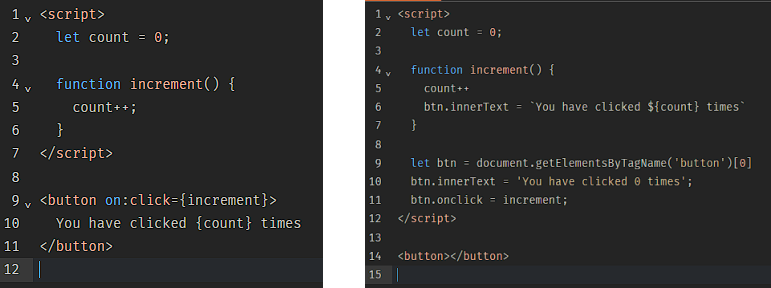
\includegraphics[width=1\textwidth]{svelte-vs-vanilla.png}
    \captionof{figure}{A button with onclick function in Svelte and vanilla JavaScript}
\end{minipage}\\\\

SvelteKit is a full-stack application framework for Svelte. It provides solutions to common problems in modern web development such as routing and server-side rendering. Documentation and interactive tutorial of Roguelighter is made with SvelteKit. \cite{sveltekit}.

\subsection{WebGL}
WebGL (Web Graphics Library) is a JavaScript API for rendering high-performance interactive 3D and 2D graphics within any compatible web browser without the use of plug-ins. WebGL does so by introducing an API that closely conforms to OpenGL ES 2.0 that can be used in HTML canvas elements. This conformance makes it possible for the API to take advantage of hardware graphics acceleration provided by the user's device \cite{webgl}. 

\subsection{ThreeJS}
ThreeJS is a canvas library which provides primitives and abstractions on top of WebGL to make building 3D projects faster, more readable, and more maintainable \cite{threejs}.

\subsection{Threlte}
Threlte is a declarative library built on top of ThreeJS. Instead of writing imperative code with ThreeJS, developers are allowed to write declarative component-based code to describe their 3D scenes \cite{threlte}.

\subsection{TypeScript}
\todo{write typescript description and features}

\subsection{HOTScript}
HOTScript is a library of composable functions for types. It uses generics to compose function-like behavior inside TypeScript’s type system \cite{hotscript}.

\subsection{TailwindCSS}
TailwindCSS is a utility-first CSS library that provides atomic classes which only affect a single CSS property . This atomic approach is inline with Roguelighter's philosophy of making things simple and local \cite{tailwindcss}.

\subsection{Monaco Editor}
Monaco Editor is an open source, fully featured, browser-based code editor. It is the editor that powers Visual Studio Code, which is the most popular integrated development environment as of today \cite{monaco-editor}\cite{developer-survey}.

\subsection{Tauri}
Tauri is a framework for building tiny and fast binaries for all major desktop platforms. Developers can integrate any front-end framework that compiles to HTML, JS and CSS for building their user interface. The backend of the application is a rust-sourced binary with an API that the front-end can interact with \cite{tauri}.

\subsection{TypeDoc}
TypeDoc is a documentation generator for TypeScript type declarations. It uses declarations themselves and TSDoc comments placed above the declarations to generate documentation in JSON or in multi page HTML format \cite{typedoc}.

\section{Architecture}
Roguelighter consists of a library and two apps. The library is the engine itself, and the apps are a desktop application and a website which includes documentation, interactive tutorial and download link for the desktop app. Library code is shared between these two projects with monorepo architecture.

\subsection{Monorepo}
Explaining monorepos can be easier if we first learn what is the opposite of a monorepo which we can name as polyrepos. A polyrepo is the current standard way of developing applications: a repo for each team, application, or project. And it's common that each repo has a single build artifact, and simple build pipeline. This approach brings autonomy to different teams working on the same project but it has its downsides.\\

First off, sharing code becomes cumbersome. The consumer repo should have a dependency to the provider repo and consumers should wait for the latest updates to go live to use a certain feature. Common code patterns and components gets implemented in each repo differently, which increases the maintenance cost for each team and creates duplicate logic. Tooling becomes inconsistent, as each team introduces their own standards or ad hoc solutions.\\

So what is a monorepo? A monorepo is a single repository containing multiple distinct projects, with well-defined relationships. No need to publish packages since all the consumers are in the same repo. No need to worry about incompatibilities because of projects depending on conflicting versions of third party libraries. Everything related to the monorepo becomes consistent whether that is a simple component, a developer tool or a complex build workflow \cite{monorepo}.

\subsection{Desktop Application}
This is where users can actually use the engine. It can be downloaded via Roguelighter's official website. \todo{explain}\\\\
\begin{minipage}{\linewidth}
    \centering
    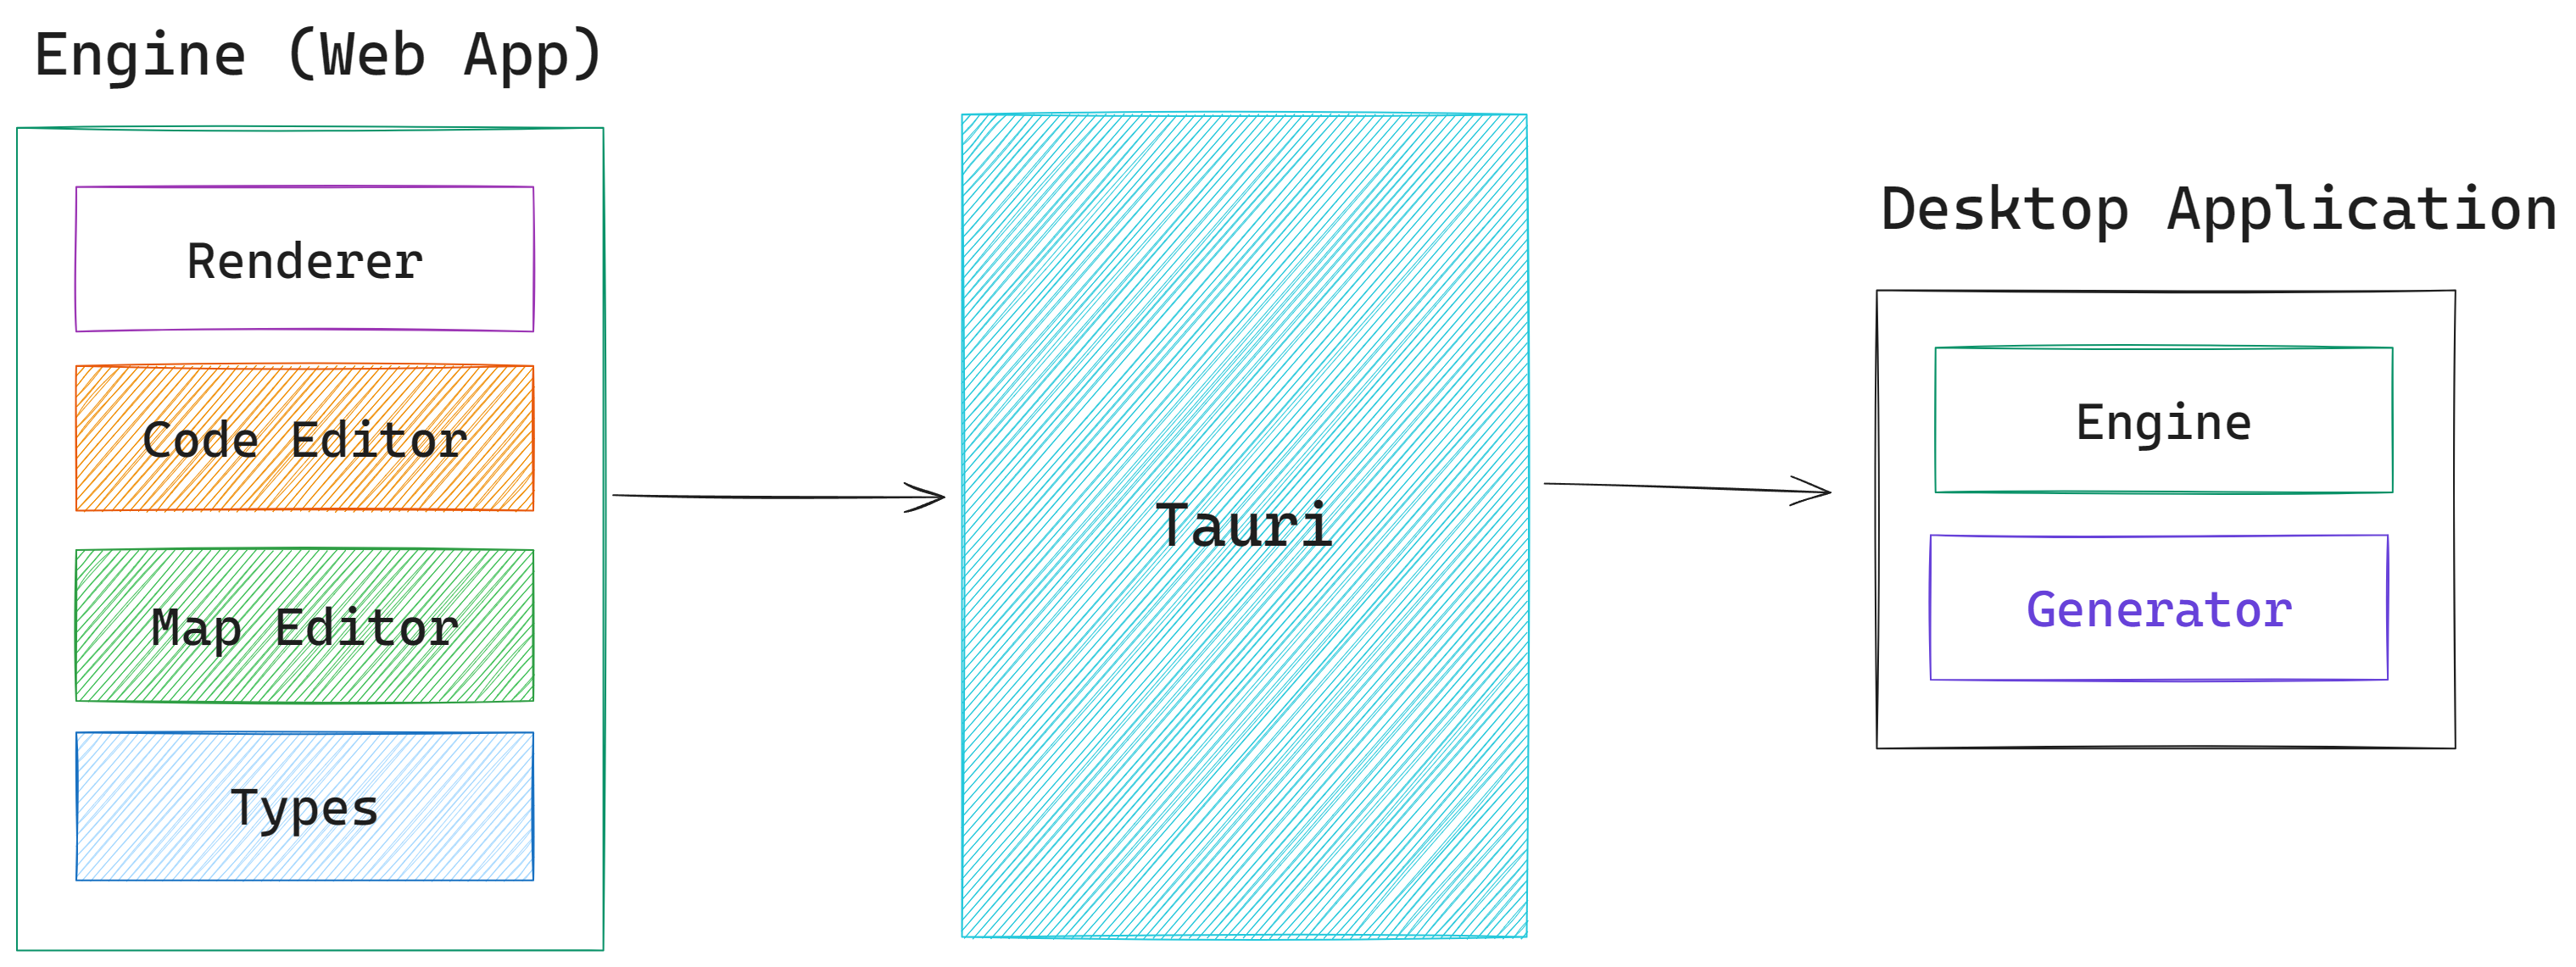
\includegraphics[width=1\textwidth]{pipeline.png}
    \captionof{figure}{Desktop application build pipeline}
\end{minipage}\\\\

\subsubsection{Components and relations}
\subsubsection{Configuration file}

\begin{itemize}
    \item \textbf{Settings:} Provides defaults for the project. Such as default frames per second, default animation function and default animation duration.\\\\
    \begin{minipage}{\linewidth}
        \centering
        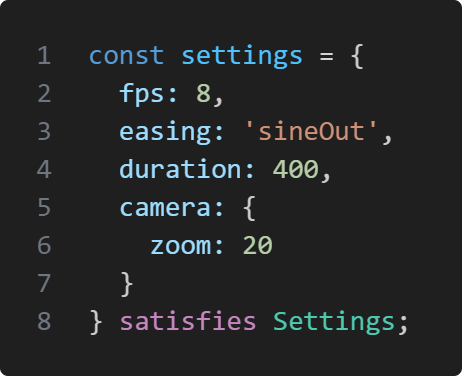
\includegraphics[width=0.5\textwidth]{settings.png}
        \captionof{figure}{Example Settings object}
    \end{minipage}\\\\
    
    \item \textbf{Backgrounds:} An object where keys define the name of the background, and value points to the route of the source. This object also affects the Map Editor interface, which we will see in \todo{reference}\\\\
    \begin{minipage}{\linewidth}
        \centering
        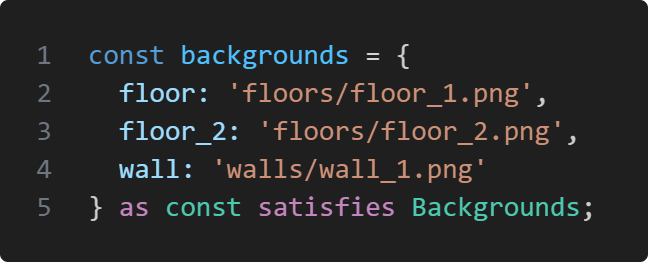
\includegraphics[width=0.7\textwidth]{backgrounds.png}
        \captionof{figure}{Example Backgrounds object}
    \end{minipage}\\\\

    \item \textbf{Collisions:} An array of background keys. This tells the game that agents cannot move into tiles with these backgrounds.\\\\
    \begin{minipage}{\linewidth}
        \centering
        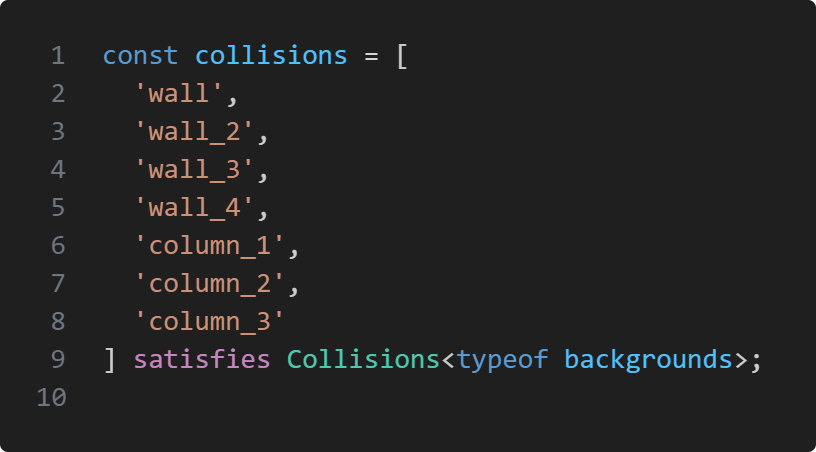
\includegraphics[width=0.7\textwidth]{collisions.png}
        \captionof{figure}{Example Collisions object}
    \end{minipage}\\\\
    
    \item \textbf{Agents:} Agents are player and non-player entities that are interactable, or have "agency". Animation states and defaults of agents can be configured in this object.\\\\
    \begin{minipage}{\linewidth}
        \centering
        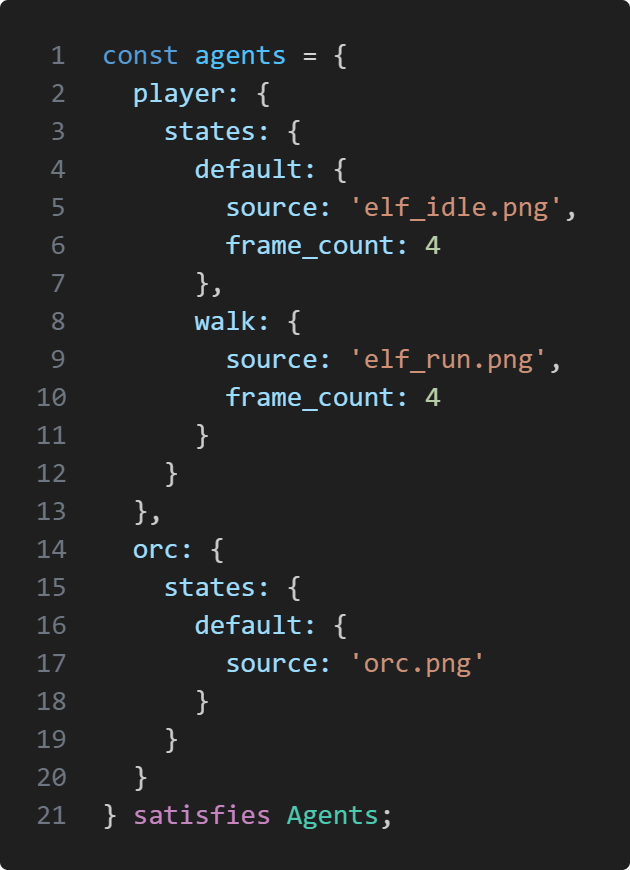
\includegraphics[width=0.5\textwidth]{agents.png}
        \captionof{figure}{Example Agents object}
    \end{minipage}\\\\
    
    \item \textbf{Variables:} These are custom variables that can be defined and manipulated by the developer via using Events \todo{refer Events}.\\\\
    \begin{minipage}{\linewidth}
        \centering
        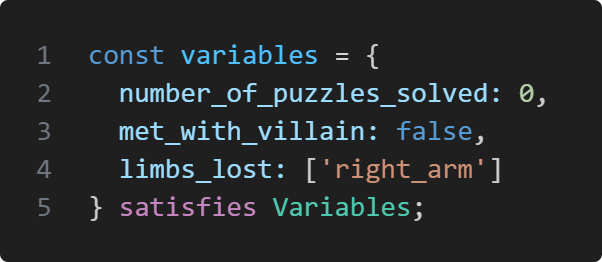
\includegraphics[width=0.5\textwidth]{variables.png}
        \captionof{figure}{Example Variables object}
    \end{minipage}\\\\
    
    \item \textbf{Events:} An object where keys define the name of the event, and values the sequence of actions (an array of arrays). An action is an array of keywords and primitive values such as strings, numbers or booleans. These values should be placed in a specific order, or the program will return a compiler error, pointing out the wrongly placed tokens. If placed correctly and required conditions are met during the game, the array of actions gets executed in order and synchronously, meaning the action will be fired once the previous action is completed.\\\\ 
        \begin{minipage}{\linewidth}
        \centering
        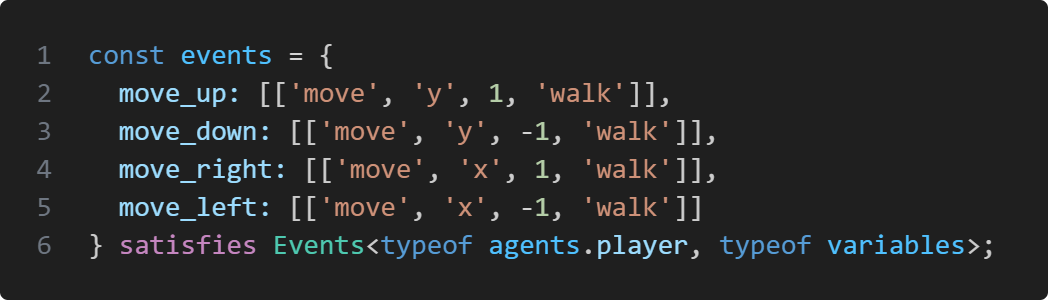
\includegraphics[width=1\textwidth]{events.png}
        \captionof{figure}{Example Events object}
    \end{minipage}\\\\
    
    \item \textbf{Key Bindings:} Keybindings is an object where the keys are codes of keyboard events such as "Escape", "ArrowUp" or "KeyF" and values are either internal events provided by the engine or keys of the Events object  \todo{refer Events}.\\\\
    \begin{minipage}{\linewidth}
        \centering
        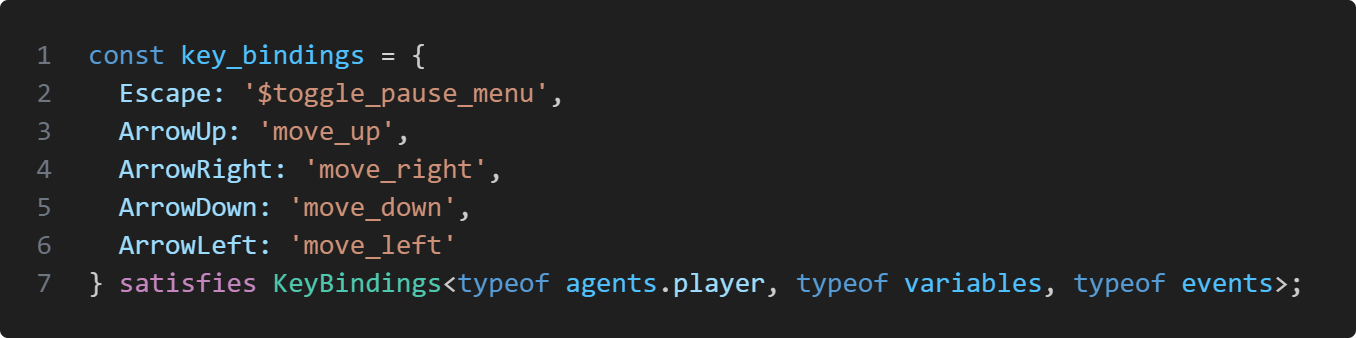
\includegraphics[width=1\textwidth]{key bindings.png}
        \captionof{figure}{Example Key Bindings object}
    \end{minipage}\\\\
    
    \item \textbf{GUI:} This object is where user defines everything related to the interface of the game whether it's a pause menu or a custom game component.\\\\
    \begin{minipage}{\linewidth}
        \centering
        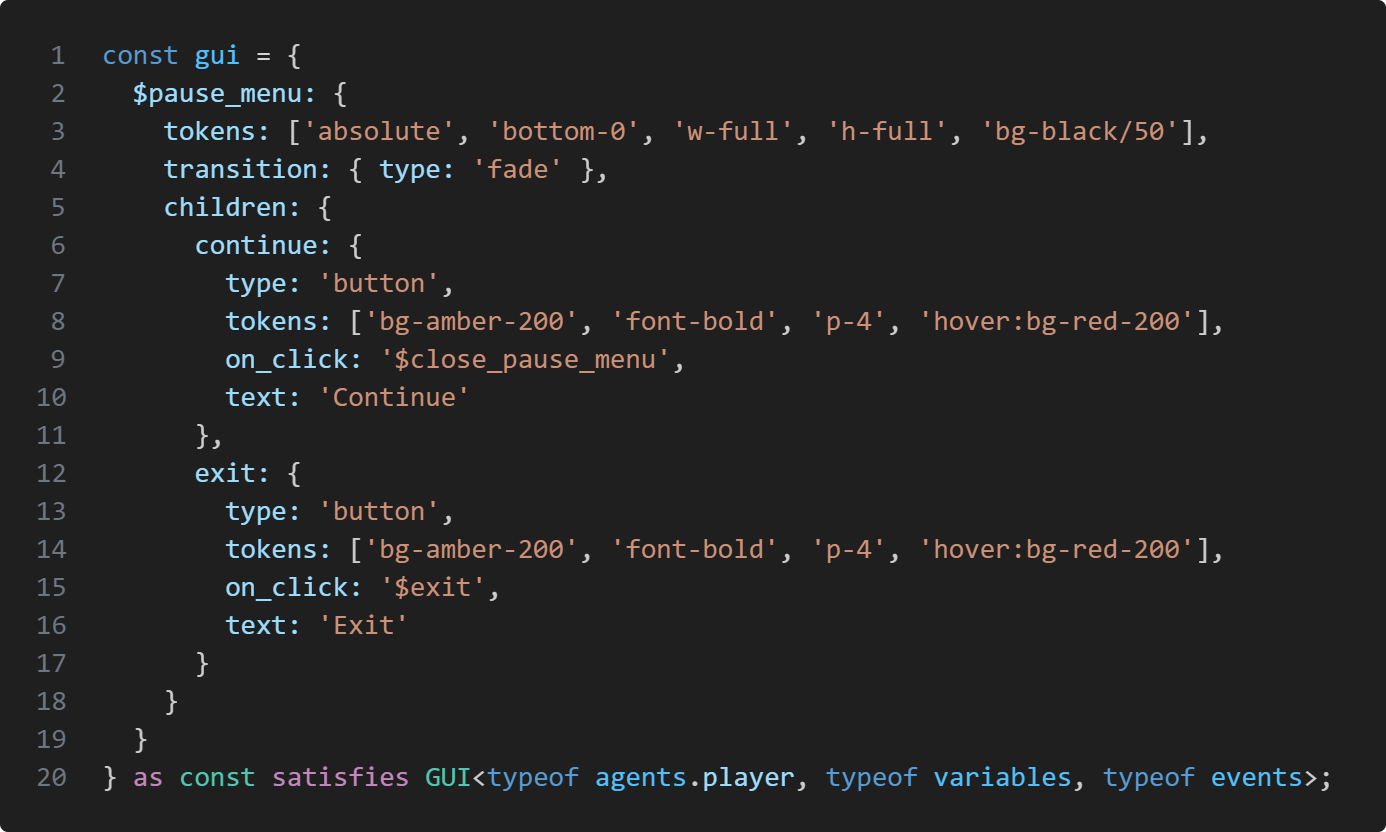
\includegraphics[width=1\textwidth]{gui.png}
        \captionof{figure}{Example GUI object}
    \end{minipage}\\\\
    
    \item \textbf{Errors:} This object is special and the only object that is not passed as an argument to the renderer. Errors object exists only to provide compile-time warnings to the developer which helps prevent run-time errors and unexpected behaviors.
\end{itemize}
\subsubsection{Views}
\begin{itemize}
    \item \textbf{Code Editor:} This is where the configuration file is edited. It defines foundations and behaviors of your game.\\

    After Svelte's onMount life-cycle function is executed, a div element inside the markup is fetched as a parameter to Monaco Editor. Once language server is loaded, the div becomes the container of the editor and ready to use. Any changes on the editor is saved into a string. This string then gets transpiled into JavaScript and fetched to the Scene Editor and Renderer as a JSON object.\\\\
    \begin{minipage}{\linewidth}
        \centering
        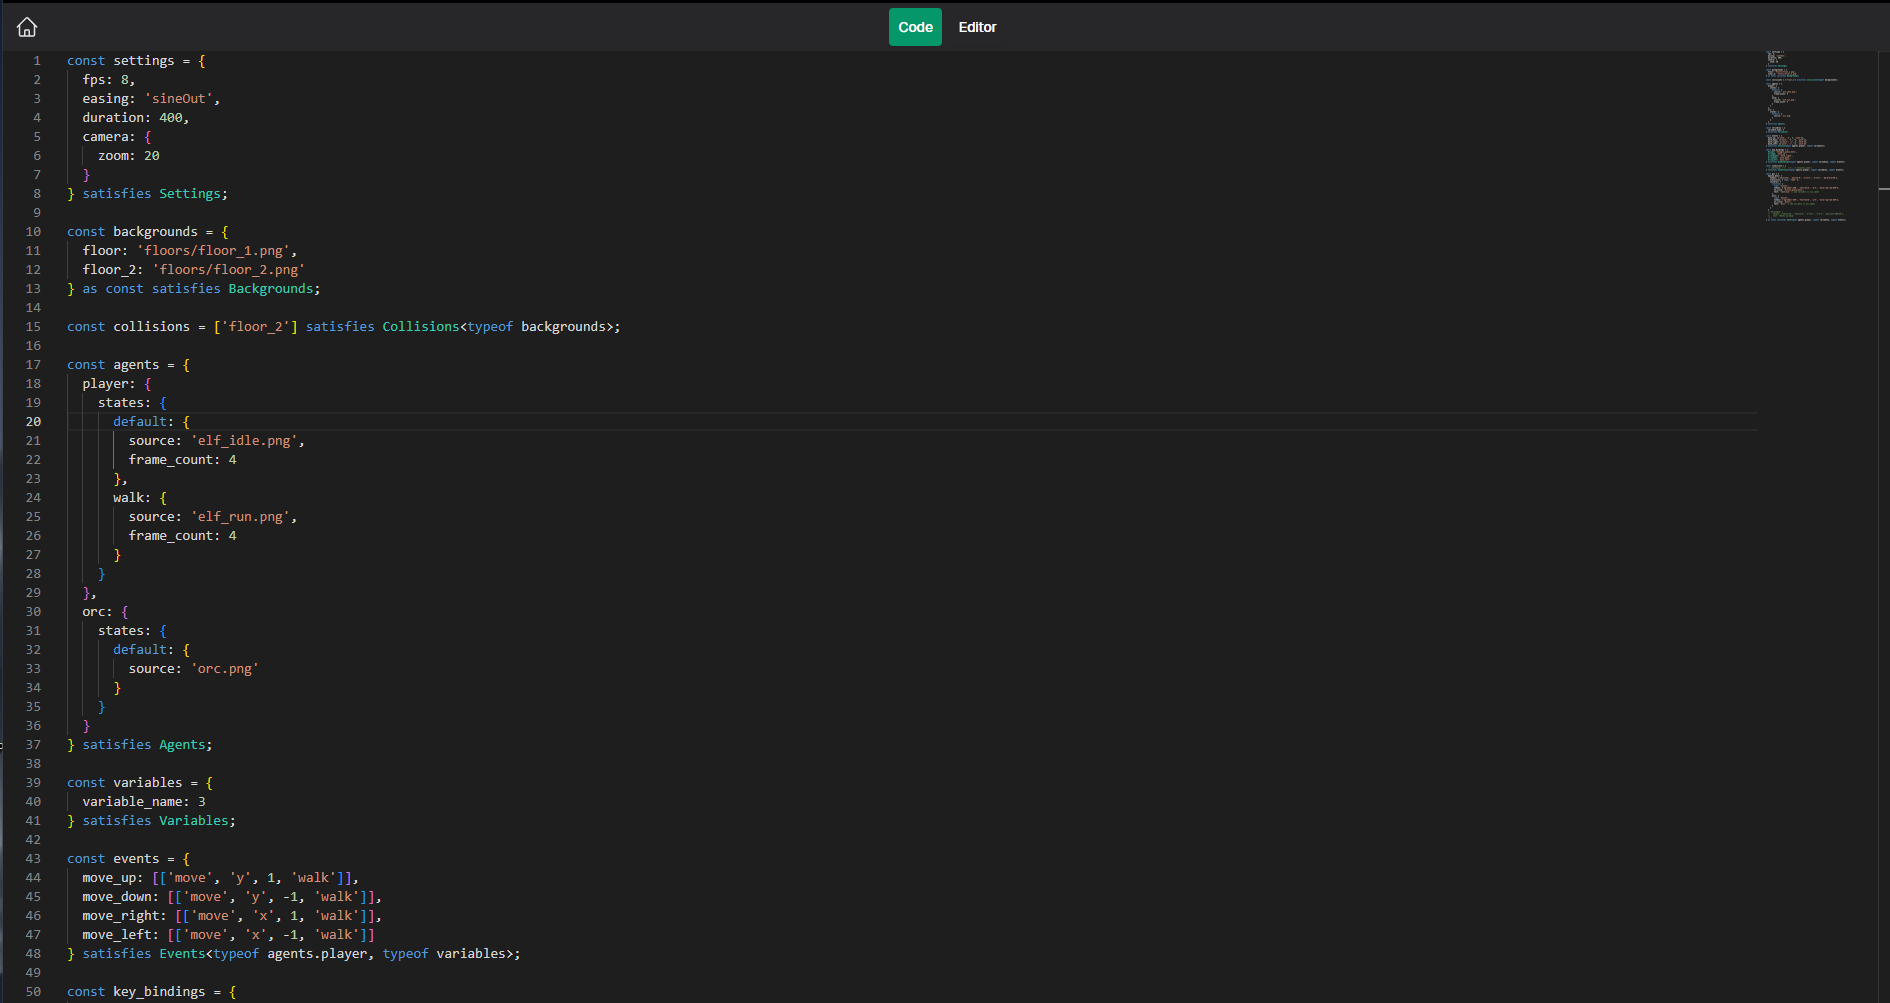
\includegraphics[width=1\textwidth]{code-editor.PNG}
        \captionof{figure}{Code Editor}
    \end{minipage}\\\\

    \item \textbf{Scene Editor:} Roguelighter games are made up of individual scenes. In Map Editor, you can create new scenes and connect them to each other by placing portals.\\
    \todo{elaborate}
    \begin{minipage}{\linewidth}
        \centering
        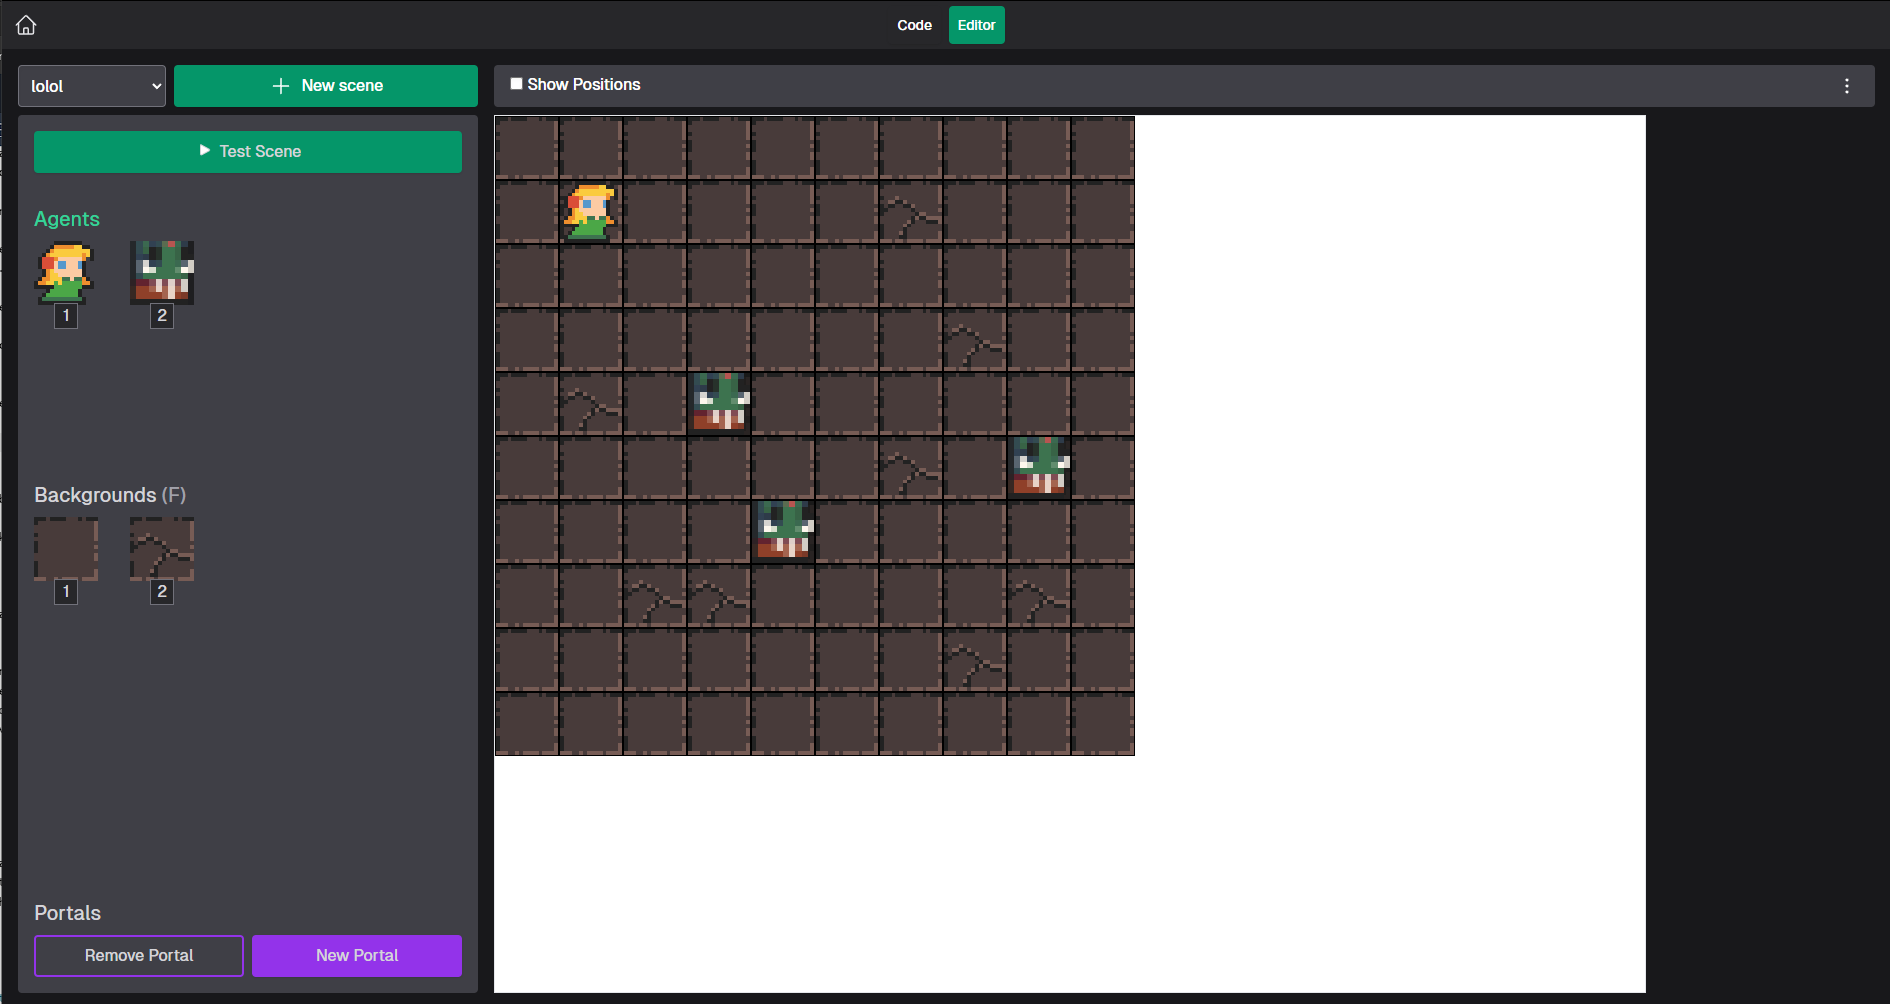
\includegraphics[width=1\textwidth]{scene-editor.PNG}
        \captionof{figure}{Scene Editor}
    \end{minipage}\\\\
    
    \item \textbf{Renderer:} This is the playground for your game, you can see how it plays out.  
\end{itemize}
\subsubsection{Exporting}
There are two options for exporting a Roguelighter project. Web or the operating system in the current machine. If the user decides to export their project into the web platform, Roguelighter generates a Svelte web application which has the Renderer from the engine, and the data provided by the user (code, scenes and assets).\\

\begin{minipage}{\linewidth}
    \centering
    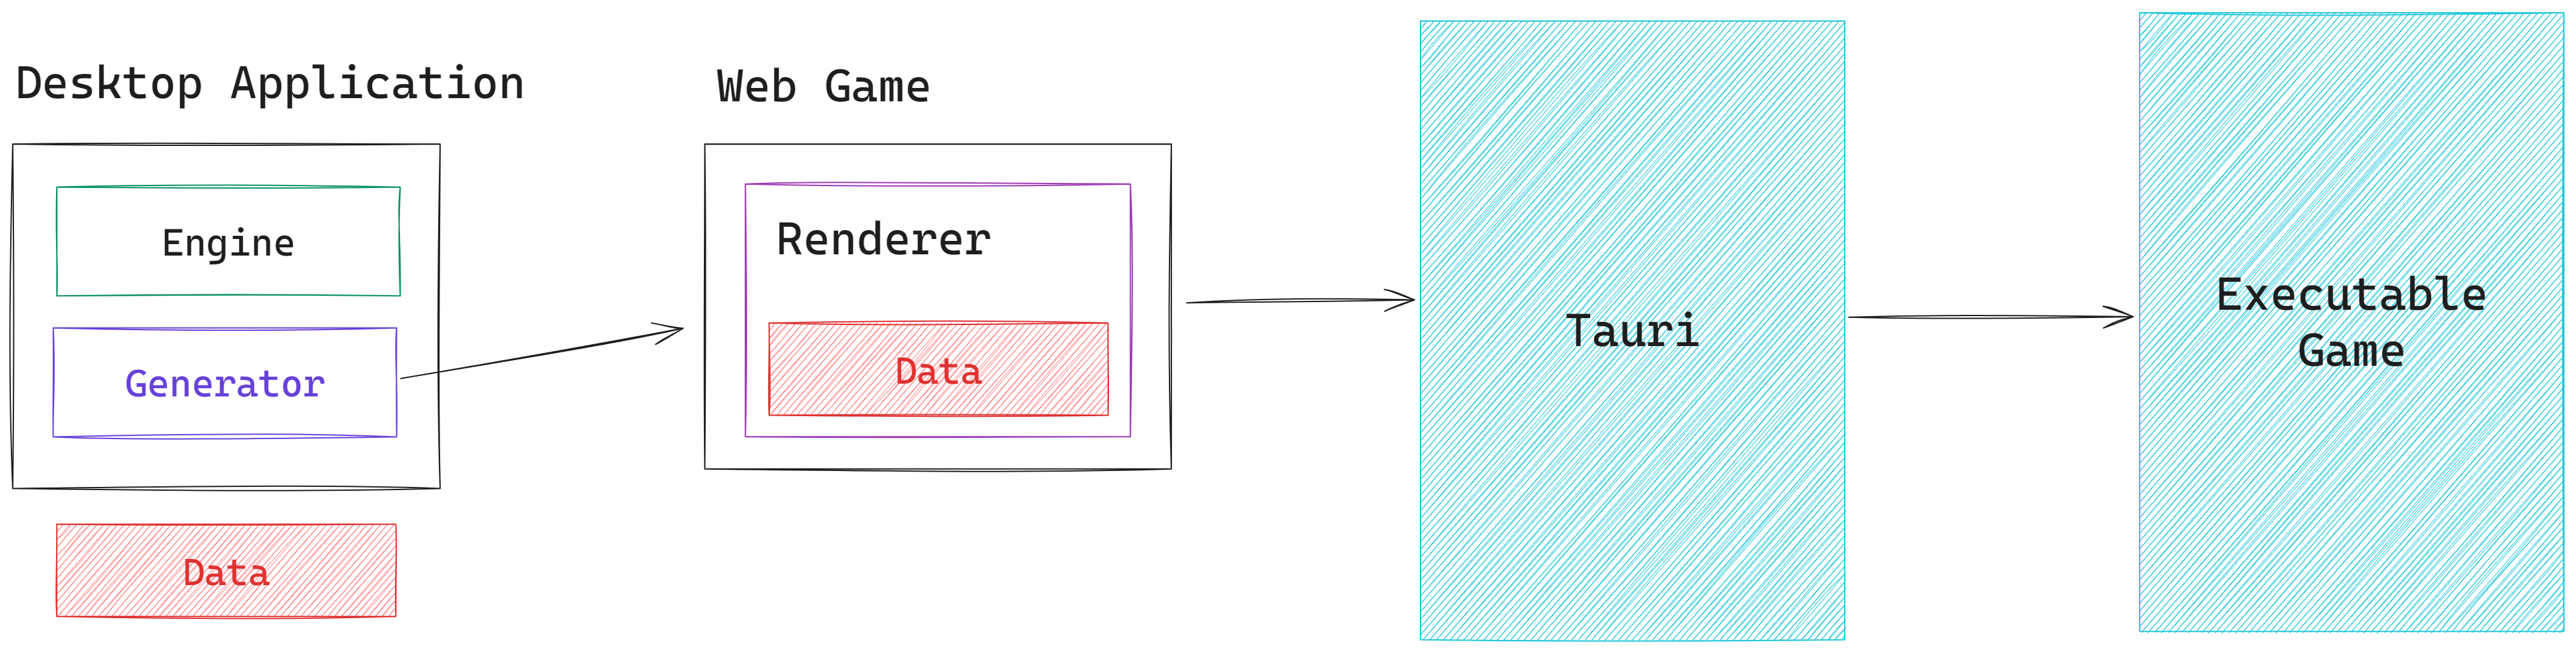
\includegraphics[width=1\textwidth]{tauri.png}
    \captionof{figure}{Exporting pipeline}
\end{minipage}\\\\

\subsection{Website}
\subsubsection{Documentation}
\subsubsection{Interactive Tutorial}

\section{Conclusion}
\subsection{Future Work}
\subsubsection{Common Roguelike Elements}
\begin{itemize}
    \item{Randomly Generated Scenes}
    \item{Inventory System}
    \item{Dialogue System}
    \item{Artificial Intelligence}
\end{itemize}
\subsubsection{TailwindCSS Language Server Integration}
The conventional way of writing Tailwind classes is inside the class attribute of an HTML element, which is basically writing a very long string. This experience can be enhanced by installing Visual Studio Code's Tailwind CSS Intellisense extension. With this extension installed, users can benefit from features such as auto-complete, syntax-highlighting and linting when writing Tailwind classes, thanks to Tailwind's language server.\\

Roguelighter has only one language server inside it and that is TypeScript's. This means the features provided by the official Tailwind extension should be replicated or discarded when writing Tailwind classes in Roguelighter's code editor.\\

Current version of Roguelighter asks the user to put tailwind class tokens in an array, each token being a separate string. We have designed it this way to provide auto-complete and type-safety for tailwind classes. Since it is not possible to parse an indefinitely long string into tokens and check if each token is a certain type at compile-time. Although this approach provides auto-complete and type-safety, it slows down writing classes and creates a lot of quotation marks and commas.\\

The alternative approach would be triggering Tailwind language server when user starts editing "tokens" property of a GUI child. This way, users would feel as if they are writing Tailwind classes inside an HTML element and get all the benefits of the official Tailwind extension for Visual Studio Code \cite{tailwind-vscode}. 
\subsubsection{Audio Support}
Audio is essential to any type of game so it should be a default feature in Roguelighter.
\printbibliography
\listoffigures
\end{document}
